%% start of file `main.tex'.
%% Copyright 2014 Francois Mouton (moutonf@gmail.com).
%
% This template is adapted from the work performed by Xavier Danaux (xdanaux@gmail.com).
% This template further extends the functionality by integrating the moderntimeline package.
% This template also includes custom Biblatex style to print bibliography items with the moderntimeline package.
%
% This work may be distributed and/or modified under the
% conditions of the LaTeX Project Public License version 1.3c,
% available at http://www.latex-project.org/lppl/.


\documentclass[11pt,a4paper,sans]{moderncv/moderncv}        % possible options include font size ('10pt', '11pt' and '12pt'), paper size ('a4paper', 'letterpaper', 'a5paper', 'legalpaper', 'executivepaper' and 'landscape') and font family ('sans' and 'roman')

% moderncv themes
\moderncvstyle{classic}                             % Only the 'classic' style is fully functional with the modifications made. The other options, 'casual' (default), 'oldstyle' and 'banking' has minor typesetting problems with the current modifications.
\moderncvcolor{blue}                               % color options 'blue' (default), 'orange', 'green', 'red', 'purple', 'grey' and 'black'
%\renewcommand{\familydefault}{\sfdefault}         % to set the default font; use '\sfdefault' for the default sans serif font, '\rmdefault' for the default roman one, or any tex font name

% character encoding
\usepackage[utf8]{inputenc}                       % if you are not using xelatex ou lualatex, replace by the encoding you are using

% adjust the page margins
\usepackage[scale=0.75]{geometry}
%\setlength{\hintscolumnwidth}{3cm}                % if you want to change the width of the column of the timeline
%\setlength{\makecvtitlenamewidth}{10cm}           % for the 'classic' style, if you want to force the width allocated to your name and avoid line breaks. Be careful though, the length is normally calculated to avoid any overlap with your personal info; use this at your own typographical risks.

%-------------------Inlcuding pdfpages package-------------------------------------------------------------

\usepackage{pdfpages/pdfpages}

%-------------------Including moderntimeline package-------------------------------------------------------

\usepackage{moderntimeline/moderntimeline}

\tlmaxdates{2004}{2014}                             % Set the scale of the timeline. \tlmaxdates{startDate}{endDate}

%-------------------Including xpatch package---------------------------------------------------------------

\usepackage{xpatch/xpatch}

%-------------------Including Biblatex package-------------------------------------------------------------

\usepackage[url=false,
    backend=biber,                                  % This can be set to either biber or bibtex. If references are missing just change back and forth between biber and bibtex..
    style=authoryear,
    doi=false,  
    isbn=false,
    backref=false,
    dashed=false,                                   % Do not add a dash out authors for subsequent articles with the same authors.
    maxnames=99,                                    % Amount of authors to include before abbreviating.
    sorting=ydnt]{biblatex}                         % Sorting in reverse order

\addbibresource{cvreferences.bib}                   % Include your bibtex file here. Format: fileName.bib

%% start of file `standard_modifications.tex'.
%% Copyright 2014 Francois Mouton (moutonf@gmail.com).
%
% This work may be distributed and/or modified under the
% conditions of the LaTeX Project Public License version 1.3c,
% available at http://www.latex-project.org/lppl/.

% remove brackets from year
\xpatchbibmacro{date+extrayear}{%
  \printtext[parens]}{\printtext}{}{}

% remove year from the author bibmacro
\xpatchbibmacro{author}{%
 \usebibmacro{date+extrayear}}
 {}{}{}

\DeclareBibliographyDriver{article}{%
  \tldatecventry{
  \thefield{year} % actual year from bibitem
  }
  {
  \usebibmacro{bibindex}%
  \usebibmacro{begentry}%
  \usebibmacro{author/translator+others}%
  \setunit{\labelnamepunct}\newblock
  \usebibmacro{title}%
  \newunit
  \printlist{language}%
  \newunit\newblock
  \usebibmacro{byauthor}%
  \newunit\newblock
  \usebibmacro{bytranslator+others}%
  \newunit\newblock
  \printfield{version}%
  \newunit\newblock
  \usebibmacro{in:}%
  \usebibmacro{journal+issuetitle}%
  \newunit
  \usebibmacro{byeditor+others}%
  \newunit
  \usebibmacro{note+pages}%
  \newunit\newblock
  \iftoggle{bbx:isbn}
    {\printfield{issn}}
    {}%
  \newunit\newblock
  \usebibmacro{doi+eprint+url}%
  \newunit\newblock
  \usebibmacro{addendum+pubstate}%
  \setunit{\bibpagerefpunct}\newblock
  \usebibmacro{pageref}%
  \newunit\newblock
  \iftoggle{bbx:related}
    {\usebibmacro{related:init}%
     \usebibmacro{related}}
    {}%
  \usebibmacro{finentry}}{}{}{}}
  
\DeclareBibliographyDriver{book}{%
  \tldatecventry{
  \thefield{year} % actual year from bibitem
  }
  {
  \usebibmacro{bibindex}%
  \usebibmacro{begentry}%
  \usebibmacro{author/editor+others/translator+others}%
  \setunit{\labelnamepunct}\newblock
  \usebibmacro{maintitle+title}%
  \newunit
  \printlist{language}%
  \newunit\newblock
  \usebibmacro{byauthor}%
  \newunit\newblock
  \usebibmacro{byeditor+others}%
  \newunit\newblock
  \printfield{edition}%
  \newunit
  \iffieldundef{maintitle}
    {\printfield{volume}%
     \printfield{part}}
    {}%
  \newunit
  \printfield{volumes}%
  \newunit\newblock
  \usebibmacro{series+number}%
  \newunit\newblock
  \printfield{note}%
  \newunit\newblock
  \usebibmacro{publisher+location+date}%
  \newunit\newblock
  \usebibmacro{chapter+pages}%
  \newunit
  \printfield{pagetotal}%
  \newunit\newblock
  \iftoggle{bbx:isbn}
    {\printfield{isbn}}
    {}%
  \newunit\newblock
  \usebibmacro{doi+eprint+url}%
  \newunit\newblock
  \usebibmacro{addendum+pubstate}%
  \setunit{\bibpagerefpunct}\newblock
  \usebibmacro{pageref}%
  \newunit\newblock
  \iftoggle{bbx:related}
    {\usebibmacro{related:init}%
     \usebibmacro{related}}
    {}%
  \usebibmacro{finentry}}{}{}{}}
  
\DeclareBibliographyDriver{booklet}{%
  \tldatecventry{
  \thefield{year} % actual year from bibitem
  }
  {
  \usebibmacro{bibindex}%
  \usebibmacro{begentry}%
  \usebibmacro{author/editor+others/translator+others}%
  \setunit{\labelnamepunct}\newblock
  \usebibmacro{title}%
  \newunit
  \printlist{language}%
  \newunit\newblock
  \usebibmacro{byauthor}%
  \newunit\newblock
  \usebibmacro{byeditor+others}%
  \newunit\newblock
  \printfield{howpublished}%
  \newunit\newblock
  \printfield{type}%
  \newunit\newblock
  \printfield{note}%
  \newunit\newblock
  \usebibmacro{location+date}%
  \newunit\newblock
  \usebibmacro{chapter+pages}%
  \newunit
  \printfield{pagetotal}%
  \newunit\newblock
  \usebibmacro{doi+eprint+url}%
  \newunit\newblock
  \usebibmacro{addendum+pubstate}%
  \setunit{\bibpagerefpunct}\newblock
  \usebibmacro{pageref}%
  \newunit\newblock
  \iftoggle{bbx:related}
    {\usebibmacro{related:init}%
     \usebibmacro{related}}
    {}%
  \usebibmacro{finentry}}{}{}{}}

\DeclareBibliographyDriver{collection}{%
  \tldatecventry{
  \thefield{year} % actual year from bibitem
  }
  {
  \usebibmacro{bibindex}%
  \usebibmacro{begentry}%
  \usebibmacro{editor+others}%
  \setunit{\labelnamepunct}\newblock
  \usebibmacro{maintitle+title}%
  \newunit
  \printlist{language}%
  \newunit\newblock
  \usebibmacro{byeditor+others}%
  \newunit\newblock
  \printfield{edition}%
  \newunit
  \iffieldundef{maintitle}
    {\printfield{volume}%
     \printfield{part}}
    {}%
  \newunit
  \printfield{volumes}%
  \newunit\newblock
  \usebibmacro{series+number}%
  \newunit\newblock
  \printfield{note}%
  \newunit\newblock
  \usebibmacro{publisher+location+date}%
  \newunit\newblock
  \usebibmacro{chapter+pages}%
  \newunit
  \printfield{pagetotal}%
  \newunit\newblock
  \iftoggle{bbx:isbn}
    {\printfield{isbn}}
    {}%
  \newunit\newblock
  \usebibmacro{doi+eprint+url}%
  \newunit\newblock
  \usebibmacro{addendum+pubstate}%
  \setunit{\bibpagerefpunct}\newblock
  \usebibmacro{pageref}%
  \newunit\newblock
  \iftoggle{bbx:related}
    {\usebibmacro{related:init}%
     \usebibmacro{related}}
    {}%
  \usebibmacro{finentry}}{}{}{}}

\DeclareBibliographyDriver{inbook}{%
  \tldatecventry{
  \thefield{year} % actual year from bibitem
  }
  {
  \usebibmacro{bibindex}%
  \usebibmacro{begentry}%
  \usebibmacro{author/translator+others}%
  \setunit{\labelnamepunct}\newblock
  \usebibmacro{title}%
  \newunit
  \printlist{language}%
  \newunit\newblock
  \usebibmacro{byauthor}%
  \newunit\newblock
  \usebibmacro{in:}%
  \usebibmacro{bybookauthor}%
  \newunit\newblock
  \usebibmacro{maintitle+booktitle}%
  \newunit\newblock
  \usebibmacro{byeditor+others}%
  \newunit\newblock
  \printfield{edition}%
  \newunit
  \iffieldundef{maintitle}
    {\printfield{volume}%
     \printfield{part}}
    {}%
  \newunit
  \printfield{volumes}%
  \newunit\newblock
  \usebibmacro{series+number}%
  \newunit\newblock
  \printfield{note}%
  \newunit\newblock
  \usebibmacro{publisher+location+date}%
  \newunit\newblock
  \usebibmacro{chapter+pages}%
  \newunit\newblock
  \iftoggle{bbx:isbn}
    {\printfield{isbn}}
    {}%
  \newunit\newblock
  \usebibmacro{doi+eprint+url}%
  \newunit\newblock
  \usebibmacro{addendum+pubstate}%
  \setunit{\bibpagerefpunct}\newblock
  \usebibmacro{pageref}%
  \newunit\newblock
  \iftoggle{bbx:related}
    {\usebibmacro{related:init}%
     \usebibmacro{related}}
    {}%
  \usebibmacro{finentry}}{}{}{}}

\DeclareBibliographyDriver{incollection}{%
  \tldatecventry{
  \thefield{year} % actual year from bibitem
  }
  {
  \usebibmacro{bibindex}%
  \usebibmacro{begentry}%
  \usebibmacro{author/translator+others}%
  \setunit{\labelnamepunct}\newblock
  \usebibmacro{title}%
  \newunit
  \printlist{language}%
  \newunit\newblock
  \usebibmacro{byauthor}%
  \newunit\newblock
  \usebibmacro{in:}%
  \usebibmacro{maintitle+booktitle}%
  \newunit\newblock
  \usebibmacro{byeditor+others}%
  \newunit\newblock
  \printfield{edition}%
  \newunit
  \iffieldundef{maintitle}
    {\printfield{volume}%
     \printfield{part}}
    {}%
  \newunit
  \printfield{volumes}%
  \newunit\newblock
  \usebibmacro{series+number}%
  \newunit\newblock
  \printfield{note}%
  \newunit\newblock
  \usebibmacro{publisher+location+date}%
  \newunit\newblock
  \usebibmacro{chapter+pages}%
  \newunit\newblock
  \iftoggle{bbx:isbn}
    {\printfield{isbn}}
    {}%
  \newunit\newblock
  \usebibmacro{doi+eprint+url}%
  \newunit\newblock
  \usebibmacro{addendum+pubstate}%
  \setunit{\bibpagerefpunct}\newblock
  \usebibmacro{pageref}%
  \newunit\newblock
  \iftoggle{bbx:related}
    {\usebibmacro{related:init}%
     \usebibmacro{related}}
    {}%
  \usebibmacro{finentry}}{}{}{}}

\DeclareBibliographyDriver{inproceedings}{%
  \tldatecventry{
  \thefield{year} % actual year from bibitem
  }
  {
  \usebibmacro{bibindex}%
  \usebibmacro{begentry}%
  \usebibmacro{author/translator+others}%
  \setunit{\labelnamepunct}\newblock
  \usebibmacro{title}%
  \newunit
  \printlist{language}%
  \newunit\newblock
  \usebibmacro{byauthor}%
  \newunit\newblock
  \usebibmacro{in:}%
  \usebibmacro{maintitle+booktitle}%
  \newunit\newblock
  \usebibmacro{event+venue+date}%
  \newunit\newblock
  \usebibmacro{byeditor+others}%
  \newunit\newblock
  \iffieldundef{maintitle}
    {\printfield{volume}%
     \printfield{part}}
    {}%
  \newunit
  \printfield{volumes}%
  \newunit\newblock
  \usebibmacro{series+number}%
  \newunit\newblock
  \printfield{note}%
  \newunit\newblock
  \printlist{organization}%
  \newunit
  \usebibmacro{publisher+location+date}%
  \newunit\newblock
  \usebibmacro{chapter+pages}%
  \newunit\newblock
  \iftoggle{bbx:isbn}
    {\printfield{isbn}}
    {}%
  \newunit\newblock
  \usebibmacro{doi+eprint+url}%
  \newunit\newblock
  \usebibmacro{addendum+pubstate}%
  \setunit{\bibpagerefpunct}\newblock
  \usebibmacro{pageref}%
  \newunit\newblock
  \iftoggle{bbx:related}
    {\usebibmacro{related:init}%
     \usebibmacro{related}}
    {}%
  \usebibmacro{finentry}}{}{}{}}

\DeclareBibliographyDriver{manual}{%
  \tldatecventry{
  \thefield{year} % actual year from bibitem
  }
  {
  \usebibmacro{bibindex}%
  \usebibmacro{begentry}%
  \usebibmacro{author/editor}%
  \setunit{\labelnamepunct}\newblock
  \usebibmacro{title}%
  \newunit
  \printlist{language}%
  \newunit\newblock
  \usebibmacro{byauthor}%
  \newunit\newblock
  \usebibmacro{byeditor}%
  \newunit\newblock
  \printfield{edition}%
  \newunit\newblock
  \usebibmacro{series+number}%
  \newunit\newblock
  \printfield{type}%
  \newunit
  \printfield{version}%
  \newunit
  \printfield{note}%
  \newunit\newblock
  \printlist{organization}%
  \newunit
  \usebibmacro{publisher+location+date}%
  \newunit\newblock
  \usebibmacro{chapter+pages}%
  \newunit
  \printfield{pagetotal}%
  \newunit\newblock
  \iftoggle{bbx:isbn}
    {\printfield{isbn}}
    {}%
  \newunit\newblock
  \usebibmacro{doi+eprint+url}%
  \newunit\newblock
  \usebibmacro{addendum+pubstate}%
  \setunit{\bibpagerefpunct}\newblock
  \usebibmacro{pageref}%
  \newunit\newblock
  \iftoggle{bbx:related}
    {\usebibmacro{related:init}%
     \usebibmacro{related}}
    {}%
  \usebibmacro{finentry}}{}{}{}}

\DeclareBibliographyDriver{misc}{%
  \tldatecventry{
  \thefield{year} % actual year from bibitem
  }
  {
  \usebibmacro{bibindex}%
  \usebibmacro{begentry}%
  \usebibmacro{author/editor+others/translator+others}%
  \setunit{\labelnamepunct}\newblock
  \usebibmacro{title}%
  \newunit
  \printlist{language}%
  \newunit\newblock
  \usebibmacro{byauthor}%
  \newunit\newblock
  \usebibmacro{byeditor+others}%
  \newunit\newblock
  \printfield{howpublished}%
  \newunit\newblock
  \printfield{type}%
  \newunit
  \printfield{version}%
  \newunit
  \printfield{note}%
  \newunit\newblock
  \usebibmacro{organization+location+date}%
  \newunit\newblock
  \usebibmacro{doi+eprint+url}%
  \newunit\newblock
  \usebibmacro{addendum+pubstate}%
  \setunit{\bibpagerefpunct}\newblock
  \usebibmacro{pageref}%
  \newunit\newblock
  \iftoggle{bbx:related}
    {\usebibmacro{related:init}%
     \usebibmacro{related}}
    {}%
  \usebibmacro{finentry}}{}{}{}}

\DeclareBibliographyDriver{online}{%
  \tldatecventry{
  \thefield{year} % actual year from bibitem
  }
  {
  \usebibmacro{bibindex}%
  \usebibmacro{begentry}%
  \usebibmacro{author/editor+others/translator+others}%
  \setunit{\labelnamepunct}\newblock
  \usebibmacro{title}%
  \newunit
  \printlist{language}%
  \newunit\newblock
  \usebibmacro{byauthor}%
  \newunit\newblock
  \usebibmacro{byeditor+others}%
  \newunit\newblock
  \printfield{version}%
  \newunit
  \printfield{note}%
  \newunit\newblock
  \printlist{organization}%
  \newunit\newblock
  \usebibmacro{date}%
  \newunit\newblock
  \iftoggle{bbx:eprint}
    {\usebibmacro{eprint}}
    {}%
  \newunit\newblock
  \usebibmacro{url+urldate}%
  \newunit\newblock
  \usebibmacro{addendum+pubstate}%
  \setunit{\bibpagerefpunct}\newblock
  \usebibmacro{pageref}%
  \newunit\newblock
  \iftoggle{bbx:related}
    {\usebibmacro{related:init}%
     \usebibmacro{related}}
    {}%
  \usebibmacro{finentry}}{}{}{}}

\DeclareBibliographyDriver{patent}{%
  \tldatecventry{
  \thefield{year} % actual year from bibitem
  }
  {
  \usebibmacro{bibindex}%
  \usebibmacro{begentry}%
  \usebibmacro{author}%
  \setunit{\labelnamepunct}\newblock
  \usebibmacro{title}%
  \newunit
  \printlist{language}%
  \newunit\newblock
  \usebibmacro{byauthor}%
  \newunit\newblock
  \printfield{type}%
  \setunit*{\addspace}%
  \printfield{number}%
  \iflistundef{location}
    {}
    {\setunit*{\addspace}%
     \printtext[parens]{%
       \printlist[][-\value{listtotal}]{location}}}%
  \newunit\newblock
  \usebibmacro{byholder}%
  \newunit\newblock
  \printfield{note}%
  \newunit\newblock
  \usebibmacro{date}%
  \newunit\newblock
  \usebibmacro{doi+eprint+url}%
  \newunit\newblock
  \usebibmacro{addendum+pubstate}%
  \setunit{\bibpagerefpunct}\newblock
  \usebibmacro{pageref}%
  \newunit\newblock
  \iftoggle{bbx:related}
    {\usebibmacro{related:init}%
     \usebibmacro{related}}
    {}%
  \usebibmacro{finentry}}{}{}{}}

\DeclareBibliographyDriver{periodical}{%
  \tldatecventry{
  \thefield{year} % actual year from bibitem
  }
  {
  \usebibmacro{bibindex}%
  \usebibmacro{begentry}%
  \usebibmacro{editor}%
  \setunit{\labelnamepunct}\newblock
  \usebibmacro{title+issuetitle}%
  \newunit
  \printlist{language}%
  \newunit\newblock
  \usebibmacro{byeditor}%
  \newunit\newblock
  \printfield{note}%
  \newunit\newblock
  \iftoggle{bbx:isbn}
    {\printfield{issn}}
    {}%
  \newunit\newblock
  \usebibmacro{doi+eprint+url}%
  \newunit\newblock
  \usebibmacro{addendum+pubstate}%
  \setunit{\bibpagerefpunct}\newblock
  \usebibmacro{pageref}%
  \newunit\newblock
  \iftoggle{bbx:related}
    {\usebibmacro{related:init}%
     \usebibmacro{related}}
    {}%
  \usebibmacro{finentry}}{}{}{}}

\DeclareBibliographyDriver{proceedings}{%
  \tldatecventry{
  \thefield{year} % actual year from bibitem
  }
  {
  \usebibmacro{bibindex}%
  \usebibmacro{begentry}%
  \usebibmacro{editor+others}%
  \setunit{\labelnamepunct}\newblock
  \usebibmacro{maintitle+title}%
  \newunit
  \printlist{language}%
  \newunit\newblock
  \usebibmacro{event+venue+date}%
  \newunit\newblock
  \usebibmacro{byeditor+others}%
  \newunit\newblock
  \iffieldundef{maintitle}
    {\printfield{volume}%
     \printfield{part}}
    {}%
  \newunit
  \printfield{volumes}%
  \newunit\newblock
  \usebibmacro{series+number}%
  \newunit\newblock
  \printfield{note}%
  \newunit\newblock
  \printlist{organization}%
  \newunit
  \usebibmacro{publisher+location+date}%
  \newunit\newblock
  \usebibmacro{chapter+pages}%
  \newunit
  \printfield{pagetotal}%
  \newunit\newblock
  \iftoggle{bbx:isbn}
    {\printfield{isbn}}
    {}%
  \newunit\newblock
  \usebibmacro{doi+eprint+url}%
  \newunit\newblock
  \usebibmacro{addendum+pubstate}%
  \setunit{\bibpagerefpunct}\newblock
  \usebibmacro{pageref}%
  \newunit\newblock
  \iftoggle{bbx:related}
    {\usebibmacro{related:init}%
     \usebibmacro{related}}
    {}%
  \usebibmacro{finentry}}{}{}{}}

\DeclareBibliographyDriver{report}{%
  \tldatecventry{
  \thefield{year} % actual year from bibitem
  }
  {
  \usebibmacro{bibindex}%
  \usebibmacro{begentry}%
  \usebibmacro{author}%
  \setunit{\labelnamepunct}\newblock
  \usebibmacro{title}%
  \newunit
  \printlist{language}%
  \newunit\newblock
  \usebibmacro{byauthor}%
  \newunit\newblock
  \printfield{type}%
  \setunit*{\addspace}%
  \printfield{number}%
  \newunit\newblock
  \printfield{version}%
  \newunit
  \printfield{note}%
  \newunit\newblock
  \usebibmacro{institution+location+date}%
  \newunit\newblock
  \usebibmacro{chapter+pages}%
  \newunit
  \printfield{pagetotal}%
  \newunit\newblock
  \iftoggle{bbx:isbn}
    {\printfield{isrn}}
    {}%
  \newunit\newblock
  \usebibmacro{doi+eprint+url}%
  \newunit\newblock
  \usebibmacro{addendum+pubstate}%
  \setunit{\bibpagerefpunct}\newblock
  \usebibmacro{pageref}%
  \newunit\newblock
  \iftoggle{bbx:related}
    {\usebibmacro{related:init}%
     \usebibmacro{related}}
    {}%
  \usebibmacro{finentry}}{}{}{}}

\DeclareBibliographyDriver{thesis}{%
  \tldatecventry{
  \thefield{year} % actual year from bibitem
  }
  {
  \usebibmacro{bibindex}%
  \usebibmacro{begentry}%
  \usebibmacro{author}%
  \setunit{\labelnamepunct}\newblock
  \usebibmacro{title}%
  \newunit
  \printlist{language}%
  \newunit\newblock
  \usebibmacro{byauthor}%
  \newunit\newblock
  \printfield{note}%
  \newunit\newblock
  \printfield{type}%
  \newunit
  \usebibmacro{institution+location+date}%
  \newunit\newblock
  \usebibmacro{chapter+pages}%
  \newunit
  \printfield{pagetotal}%
  \newunit\newblock
  \iftoggle{bbx:isbn}
    {\printfield{isbn}}
    {}%
  \newunit\newblock
  \usebibmacro{doi+eprint+url}%
  \newunit\newblock
  \usebibmacro{addendum+pubstate}%
  \setunit{\bibpagerefpunct}\newblock
  \usebibmacro{pageref}%
  \newunit\newblock
  \iftoggle{bbx:related}
    {\usebibmacro{related:init}%
     \usebibmacro{related}}
    {}%
  \usebibmacro{finentry}}{}{}{}}

\DeclareBibliographyDriver{unpublished}{%
  \tldatecventry{
  \thefield{year} % actual year from bibitem
  }
  {
  \usebibmacro{bibindex}%
  \usebibmacro{begentry}%
  \usebibmacro{author}%
  \setunit{\labelnamepunct}\newblock
  \usebibmacro{title}%
  \newunit
  \printlist{language}%
  \newunit\newblock
  \usebibmacro{byauthor}%
  \newunit\newblock
  \printfield{howpublished}%
  \newunit\newblock
  \printfield{note}%
  \newunit\newblock
  \usebibmacro{location+date}%
  \newunit\newblock
  \iftoggle{bbx:url}
    {\usebibmacro{url+urldate}}
    {}%
  \newunit\newblock
  \usebibmacro{addendum+pubstate}%
  \setunit{\bibpagerefpunct}\newblock
  \usebibmacro{pageref}%
  \newunit\newblock
  \iftoggle{bbx:related}
    {\usebibmacro{related:init}%
     \usebibmacro{related}}
    {}%
  \usebibmacro{finentry}}{}{}{}}

\DeclareBibliographyDriver{shorthand}{%
  \tldatecventry{
  \thefield{year} % actual year from bibitem
  }
  {
  \usedriver
    {\DeclareNameAlias{sortname}{default}}
    {\thefield{entrytype}}%
  \finentry}{}{}{}}

\DeclareBibliographyDriver{set}{%
  \tldatecventry{
  \thefield{year} % actual year from bibitem
  }
  {
  \entryset{}{}%
  \newunit\newblock
  \usebibmacro{setpageref}%
  \finentry}{}{}{}}
  
%% end of file `standard_modification.tex'.        % Modifying the default standard.tex style of Biblatex. This modification is performed to include the moderntimeline package.

%-------------------Defining a CV Reference column style and a CV reference entry block-------------------

% Adapted from the solution provided in: http://tex.stackexchange.com/questions/34881/references-section-in-a-cv
% usage: \cvreference{name}{address line 1}{address line 2}{address line 3}{address line 4}{e-mail address}{phone number}{mobile phone number}
% Everything but the name is optional
% If \addresssymbol, \emailsymbol or \phonesymbol are specified, they will be used.
% (Per default, \addresssymbol isn't specified, the other two are specified.)
% If you don't like the symbols, remove them from the following code, including the tilde ~ (e.g. \phonesymbol~).

\newcommand{\cvreferencecolumn}[2]{%
  \cvitem[0.75em]{}{%
    \begin{minipage}[t]{\listdoubleitemmaincolumnwidth}#1\end{minipage}%
    \hfill%
    \begin{minipage}[t]{\listdoubleitemmaincolumnwidth}#2\end{minipage}%
    }%
}

\newcommand{\cvreference}[8]{%
    \textbf{#1}\newline% Name
    \ifthenelse{\equal{#2}{}}{}{\addresssymbol~#2\newline}%
    \ifthenelse{\equal{#3}{}}{}{#3\newline}%
    \ifthenelse{\equal{#4}{}}{}{#4\newline}%
    \ifthenelse{\equal{#5}{}}{}{#5\newline}%
    \ifthenelse{\equal{#6}{}}{}{\emailsymbol~\texttt{\href{mailto:#6}{\nolinkurl{#6}}}\newline}%
    \ifthenelse{\equal{#7}{}}{}{\phonesymbol~#7\newline}
    \ifthenelse{\equal{#8}{}}{}{\mobilephonesymbol~#8}}

%-------------------Personal Data for CV title-----------------------------------------------------------
% Example:
% \name{John}{Doe}
% \title{Resumé title}                               % optional, remove / comment the line if not wanted
% \address{street and number}{postcode city}{country}% optional, remove / comment the line if not wanted; the "postcode city" and and "country" arguments can be omitted or provided empty
% \phone[mobile]{+1~(234)~567~890}                   % optional, remove / comment the line if not wanted
% \phone[fixed]{+2~(345)~678~901}                    % optional, remove / comment the line if not wanted
% \phone[fax]{+3~(456)~789~012}                      % optional, remove / comment the line if not wanted
% \email{john@doe.org}                               % optional, remove / comment the line if not wanted
% \homepage{www.johndoe.com}                         % optional, remove / comment the line if not wanted
% \extrainfo{additional information}                 % optional, remove / comment the line if not wanted
% \photo[64pt][0.4pt]{picture}                       % optional, remove / comment the line if not wanted; '64pt' is the height the picture must be resized to, 0.4pt is the thickness of the frame around it (put it to 0pt for no frame) and 'picture' is the name of the picture file stored
% \quote{Some quote}                                 % optional, remove / comment the line if not wanted


\name{Francois}{Mouton}
\title{Curriculum Vit\ae{}}                         % optional, remove / comment the line if not wanted
\address{716 Makou Street\\Monument Park\\Pretoria}{0181}{South Africa}% optional, remove / comment the line if not wanted; the "postcode city" and and "country" arguments can be omitted or provided empty
\phone[mobile]{+27~(82)~857~5842}                   % optional, remove / comment the line if not wanted
\phone[fixed]{+27~(12)~841~2242}                    % optional, remove / comment the line if not wanted
% \phone[fax]{+3~(456)~789~012}                     % optional, remove / comment the line if not wanted
\email{moutonf@gmail.com}                           % optional, remove / comment the line if not wanted
\homepage{www.social-engineer.co.za}                % optional, remove / comment the line if not wanted
% \extrainfo{additional information}                % optional, remove / comment the line if not wanted
\photo[64pt][0.4pt]{images/picture}                 % optional, remove / comment the line if not wanted; '64pt' is the height the picture must be resized to, 0.4pt is the thickness of the frame around it (put it to 0pt for no frame) and 'picture' is the name of the picture file
% \quote{Some quote}                                % optional, remove / comment the line if not wanted

%-------------------------------------------------------------------------------------------------------
%   Content
%-------------------------------------------------------------------------------------------------------
\begin{document}

%-------------------Cover letter------------------------------------------------------------------------

%% start of file `coverletter.tex'.
%% Copyright 2014 Francois Mouton (moutonf@gmail.com).
%
% This template is adapted from the work performed by Xavier Danaux (xdanaux@gmail.com).
%
% This work may be distributed and/or modified under the
% conditions of the LaTeX Project Public License version 1.3c,
% available at http://www.latex-project.org/lppl/.

%example:
% \recipient{Company Recruitment team}{Company, Inc.\\123 somestreet\\some city}
% \date{January 01, 1984}
% \opening{Dear Sir or Madam,}
% \closing{Yours faithfully,}
% \enclosure[Attached]{curriculum vit\ae{}}          % use an optional argument to use a string other than "Enclosure", or redefine %\enclname
% \makelettertitle
%
% Lorem ipsum dolor sit amet, consectetur adipiscing elit. Duis ullamcorper neque sit amet lectus facilisis sed luctus nisl iaculis. Vivamus at neque arcu, sed tempor quam. Curabitur pharetra tincidunt tincidunt. Morbi volutpat feugiat mauris, quis tempor neque vehicula volutpat. Duis tristique justo vel massa fermentum accumsan. Mauris ante elit, feugiat vestibulum tempor eget, eleifend ac ipsum. Donec scelerisque lobortis ipsum eu vestibulum. Pellentesque vel massa at felis accumsan rhoncus.
% 
% Suspendisse commodo, massa eu congue tincidunt, elit mauris pellentesque orci, cursus tempor odio nisl euismod augue. Aliquam adipiscing nibh ut odio sodales et pulvinar tortor laoreet. Mauris a accumsan ligula. Class aptent taciti sociosqu ad litora torquent per conubia nostra, per inceptos himenaeos. Suspendisse vulputate sem vehicula ipsum varius nec tempus dui dapibus. Phasellus et est urna, ut auctor erat. Sed tincidunt odio id odio aliquam mattis. Donec sapien nulla, feugiat eget adipiscing sit amet, lacinia ut dolor. Phasellus tincidunt, leo a fringilla consectetur, felis diam aliquam urna, vitae aliquet lectus orci nec velit. Vivamus dapibus varius blandit.
% 
% Duis sit amet magna ante, at sodales diam. Aenean consectetur porta risus et sagittis. Ut interdum, enim varius pellentesque tincidunt, magna libero sodales tortor, ut fermentum nunc metus a ante. Vivamus odio leo, tincidunt eu luctus ut, sollicitudin sit amet metus. Nunc sed orci lectus. Ut sodales magna sed velit volutpat sit amet pulvinar diam venenatis.
%
% Albert Einstein discovered that $e=mc^2$ in 1905.
%
% \[ e=\lim_{n \to \infty} \left(1+\frac{1}{n}\right)^n \]
%
% \makeletterclosing
%
% \clearpage



\recipient{To whom it may concern}{}
\date{\today}
\opening{Dear Sir or Madam,}
\closing{Yours faithfully,}
\enclosure[Attached]{curriculum vit\ae{}}          % use an optional argument to use a string other than "Enclosure", or redefine \enclname

\makelettertitle

I would like to take this opportunity to introduce myself, \textbf{Francois Mouton}.

I obtained my BSc Computer Science degree from the University of Pretoria in 2007. As part of this BSc Computer Science degree I also completed all the financial accounting subjects as required for a Bcom degree in order to have a sufficient accounting background. In 2008 I obtained my BSc Computer Science (Honours) degree and in 2012 I obtained my MSc Computer Science degree with distinction also at the University of Pretoria. Along with my MSc Computer Science degree, I also completed all of the undergraduate BA Psychology and Research subjects in order to form a basis for my PhD research in Social Engineering. I also attended an A+ Technician Course from Damelin College in 2004. Currently I am studying towards my PhD Computer Science degree.

During my student years I was employed by the University of Pretoria as an assistant lecturer for undergraduate and postgraduate courses in: Digital Forensics, Computer Security, Computer Networks and Databases.

I was previously employed as an administrator and developer at Abacus Recruitment. I also performed work for Shaya and Cyanre as a digital forensic investigator on a contractual basis. I started working at the CSIR in November, 2011. 

I am part of the Information and Computer Security Architecture research group at the University of Pretoria. At this research group I performed extensive research on security, network attacks and digital forensic readiness in a wireless sensor network domain. I am also supervising MSc and honours students at the University of Pretoria within the field of Social Engineering.

I am currently still employed at the CSIR (Council for Scientific and Industrial Research), in the operating unit of Defence Peace, Safety and Security under the Command, Control and Information Warfare competency area. I am a principle developer on several projects on cyber security, digital forensics and mobile security for the South African defence force.

\makeletterclosing

\clearpage

%% end of file `coverletter.tex'.                             % Include cover letter from coverletter.tex

%-------------------Resume------------------------------------------------------------------------------

\makecvtitle

%-------------------Education Section-------------------------------------------------------------------

\section{Education}

% For a date range: (To indicate 'up to present', set EndYear to 0)
% Format:  \tlcventry{StartYear}{EndYear}{Degree}{Institution}{City}{\textit{Grade}}{Description}  % Arguments 3 (Degree) to 6 (Grade) can be left empty. 
% Example: \tlcventry{2012}{0}{BSc Computer Science}{University of MyCity}{MyCity}{}{Also completed several random courses}

% For a single year:
% Format:  \tldatecventry{StartYear}{Degree}{Institution}{City}{\textit{Grade}}{Description}
% Example: \tldatecventry{2008}{Senior Certificate}{High School MyCity}{MyCity}{\textit{80\%}}{Passed with distinction}

%-------------------In Progress Education---------------------------------------------------------------

\subsection{In Progress}

\tlcventry{2012}{0}{PhD Computer Science}{University of Pretoria}{Pretoria}{}{Social Engineering Prevention and Awareness}

%-------------------Completed Education-----------------------------------------------------------------

\subsection{Completed}

\tlcventry{2009}{2012}{MSc Computer Science (Cum Laude)}{University of Pretoria}{Pretoria}{}{Additionally, completed all undergraduate Psychology and Research modules in preperation for PhD}
\tldatecventry{2008}{BSc Computer Science Honours}{University of Pretoria}{Pretoria}{}{}
\tldatecventry{2008}{IFIP-TC6 Summer School on Wireless Computing}{University of Pretoria}{Pretoria}{}{}
\tlcventry{2005}{2007}{BSc Computer Science}{University of Pretoria}{Pretoria}{}{Additionally, completed all undergraduate Financial Accounting modules}
\tldatecventry{2004}{Senior Certificate (Distinction)}{High School Outeniqua}{George}{}{}
\tldatecventry{2004}{A+ Technician Course (Distinction)}{Damelin}{George}{}{}

%-------------------PhD Thesis Section------------------------------------------------------------------

\section{PhD thesis}

% Format:  \cvitem{Section Name}{Description}
% Example: \cvitem{title}{\emph{The title of my PhD goes here}}
% Example: \cvitem{supervisors}{My supervisors' names go here}
% Example: \cvitem{description}{Short thesis abstract}

\cvitem{title}{\emph{Social Engineering Prevention and Awareness}}
\cvitem{supervisors}{Prof H.S. Venter, Dr L. Leenen}
\cvitem{description}{The goal of this research is to further define social engineering and develop attack detection models for social engineering. In order to perform this research, ethical requirements for performing social engineering research are developed. During this research several assisting components are developed: An ontological model for social engineering, a social engineering attack framework and social engineering awareness measurements. Furthermore, social engineering attack detection models are developed for bidirectional communication, uni-directional communication and indirect communication. Using the attack detection models the goal is to improve an individual's resilience against social engineering attacks.}

%-------------------Masters Thesis Section--------------------------------------------------------------

\section{Master thesis}

% Format:  \cvitem{Section Name}{Description}
% Example: \cvitem{title}{\emph{The title of my Masters goes here}}
% Example: \cvitem{supervisors}{My supervisors' names go here}
% Example: \cvitem{description}{Short thesis abstract}

\cvitem{title}{\emph{Digital forensic readiness for wireless sensor network environments}}
\cvitem{supervisor}{Prof H.S. Venter}
\cvitem{description}{The contribution of this research is the digital forensic readiness prototype that can be used to add a digital forensics layer to any existing wireless sensor network. The prototype ensures the integrity and authenticity of each of the data packets captured from the wireless sensor network by using the number of nodes in the network that have seen the specific data packet. The prototype does not require any modification to be made on the existing wireless sensor network and is deployed as an additional wireless sensor network. One of the main problems in wireless sensor networks is flooding attacks. The prototype is able to detect flooding attacks and immediately alerts the user and pinpoints the origin of the flooding attack.}

%-------------------Achievements Section----------------------------------------------------------------

\section{Achievements}

% Format:  \cvlistitem{Achievement}
% Example: \cvlistitem{Completed 4 marathons}
% Example: \cvlistitem{Another achievement. This achievement is particularly long and therefore normally spans over several lines. Did you notice the indentation when the line wraps?}

\cvlistitem{Member of the Golden Key Honours Society since 2007.}
\cvlistitem{One of the top second year students performing the BSc Computer Science degree.}
\cvlistitem{Received two awards for the final year project in BSc Computer Science. They are respectively Most Viable Business Opportunity and Most Profound Scientific Development Approach.}
\cvlistitem{Masters thesis forms part of the IT- and Forensic Knowledgebase DVD for the German Federal Police and is supported by INTERPOL, EUROPOL and several academic institutions around the world.}
\cvlistitem{Invited speaker for the Enterprise Mobility Conference 2014 and presented on Managing and securing our network in the virtual cloud.}
\cvlistitem{Invited to chair a panel discussion at the Information Security South Africa 2014 conference on ethical concerns regarding social engineering.}
\cvlistitem{Performed a radio interview on the data breach of the whistle blower website of the South African Police Services.}
\cvlistitem{Developed an academic \LaTeX{} template utilising the moderncv package and the moderntimeline package and implemented automated BibTeX references.} 
\cvlistitem{Helped out at Electronic Sports World Cup and World Cyber Games Preliminaries to manage the competition and maintain the network throughout the competition.}
\cvlistitem{Completed the Ekman Micro Expression Training Tool Advanced course.}

%-------------------Languages Section-------------------------------------------------------------------

\section{Languages}

% Format:  \cvitemwithcomment{Language}{Skill level}{Comment}
% Example: \cvitemwithcomment{English}{Native}{Mother Tongue}
% Example: \cvitemwithcomment{French}{Fluent}{Daily practice, all work performed in English}

\cvitemwithcomment{Afrikaans}{Native}{Mother Tongue}
\cvitemwithcomment{English}{Fluent}{Daily practice, all work performed in English}

%-------------------Interests Section-------------------------------------------------------------------

\section{Interests}

% Format:  \cvitem{Hobby}{Description}
% Example: \cvitem{Gaming}{Computer Games}
% Example: \cvitem{Sport}{Golf, Tennis}

\cvitem{Gaming}{Board Games, Competitive Trading Card Games, Computer Games, Poker}
\cvitem{Sports}{Adventure Golf, Disc Golf, Formula One}
\cvitem{Reality Shows}{Amazing Race, Masterchef, Survivor}

%-------------------Workshops Presented Section---------------------------------------------------------

\section{Workshops Presented}

\tlcventry{2008}{2011}{Hands-on ethical hacking and software security}{Information Security South Africa}{Johannesburg}{}{Presented annually}

%-------------------Experience Section------------------------------------------------------------------

\section{Experience}

%-------------------Vocational Experience---------------------------------------------------------------

\subsection{Vocational}

% Format: \tlcventry{StartYear}{EndYear}{Job title}{Employer}{City}{Country (optional)}{General description no longer than 1--2 lines.\newline{}%
% Example:
% \tlcventry{2008}{2011}{System Administrator}{Simple Solutions}{MyCity}{}{Did system administrative work.\newline{}%
% Main Duties:%
%  \begin{itemize}%
%      \item Administrate the servers;
%      \item Administrate employee computers 
%          \begin{itemize}%
%              \item All employee's computers had to be up to date;
%          \end{itemize}
%      \item Did some more administrating
%   \end{itemize}}
   
% November 2011 to Date
\tlcventry{2011}{0}{Information Warfare Specialist}{Council for Scientific and Industrial Research}{Pretoria}{}{Principle developer on several projects on cyber security, digital forensics and mobile security for the South African defence force. Work within the CSIR is considered restricted and as such cannot be written about in depth.\newline{}%
Tasks and Projects:%
\begin{itemize}%
\item Authored user manuals for applied research applications;
\item Developed applications to perform specialised network attacks and reconnaissance;
\item Developed applications to harvest public data and perform topic modelling on the data;
\item Developed a framework to perform remote network reconnaissance and web based exploitations;
\item Investigated hardware and software platforms to determine approved devices for specialist client needs;
\item Developed a digital video for security awareness of scholars and young adults;
\item Developed malware for the Android operating system;
\item Developed and ported hacking tools from a Unix based system to the Android operating system;
\item Developed a web based GPU password cracking application;
\item Developed security awareness applications to be used by the client;
\item Developed a network monitoring tool to determine the layout of the network and to predict network attacks;
\item Developed a policy to prevent social engineering in the CSIR environment;
\item Developed facial recognition software using the OpenCV framework;
\item Presented cyber security awareness to staff on the CSIR campus;
\item Developed an application to determine the level of security awareness of an individual;
\item Developed a web based application to authorise devices connecting to an access point;
\item Developed cyber security challenges for the annual penetration testing competition; and
\item Performed penetration tests on the client's network and server infrastructure.
\end{itemize}
Main duties:%
\begin{itemize}%
\item Author proposals for research projects in line with the needs of the client;
\item Actively take part and present at research seminars and research conferences;
\item Performed duties as the head of the social committee;
\item Perform collaborative research with university and industry;
\item Drafted contracts and obtained external funding to perform research projects;
\item Supervised students at the university in their masters degrees;
\item Actively engage with universities and present guest lectures;
\item Maintained own professional development as a researcher;
\item Developed several projects as the principle developer;
\item Actively take part in external committees such as the ICSA (Information and computer security architecture) research group; 
\item Acted as project lead on several projects and lead the project development cycle; and
\item Improved the RD\&I processes at the CSIR in significant ways to improve on the turnaround time of projects.
\end{itemize}}

\tlcventry{2006}{2011}{Assistant Lecturer}{University of Pretoria}{Pretoria}{}{Presented lectures and practical subjects in the fields of Computer Security and Digital Forensics. Progressed from being a tutor to the position of assistant lecturer.\newline{}%
Detailed positions:%
\begin{itemize}%
\item Assistant Lecturer for Digital Forensics (Postgraduate);
\item Assistant Lecturer for Computer Security (Postgraduate \& Undergraduate);
\item Research Assistant on Wireless Sensor Networks;
\item Head Tutor for Computer Security (Postgraduate);
\item Assistant Lecturer for Computer Networks (Undergraduate);
\item Assistant Lecturer for Databases (Undergraduate);
\item Head Tutor for Concurrent Systems (Undergraduate);
\item Head Tutor for Operating Systems (Undergraduate); and
\item Tutor for C\# Programming (Undergraduate).
\end{itemize}
Main duties:%
\begin{itemize}%
\item Prepared and presented practical sessions on the specified field of the subject;
\item Assisted students with learning activities and provided technical assistance where necessary;
\item Participated in the development, administration and marking of exams and other assessments;
\item Developed novel computer security assignments based on my expertise within the field;
\item Developed digital forensic investigation crime scenes for practical exercises based on work experience within the field;
\item Encouraged students to participate in international security challenges and provided guidance with challenges;
\item Supervised student groups who had to perform final year projects for degree purposes; and
\item Assisted in the development of learning material.
\end{itemize}}

% October 2011 to November 2011
\tldatelabelcventry{2011}{October 2011}{Digital Forensic Investigator}{CYANRE}{Centurion}{}{Performed digital forensic investigations for external clients.\newline{}%
Main duties:%
\begin{itemize}%
\item Performed acquisitions of digital evidence from several different types of digital media;
\item Performed analysis on digital evidence and identify what activity has occurred on the digital evidence;
\item Authored comprehensive reports which presented the facts obtained during the analysis phase; and
\item Ensured that a chain of custody of all the evidence items is kept at all times.
\end{itemize}}

% July 2010 to November 2010
\tldatecventry{2010}{Digital Forensic Investigator}{SHAYA}{Johannesburg}{}{Performed digital forensic investigations for external clients and developed internal software.\newline{}%
Main duties:%
\begin{itemize}%
\item Performed acquisitions of digital evidence from several different types of digital media;
\item Performed data recovery on digital media;
\item Performed analysis on digital evidence and identify what activity has occurred on the digital evidence;
\item Authored comprehensive reports which presented the facts obtained during the analysis phase;
\item Ensured that a chain of custody of all the evidence items is kept at all times; and
\item Developed internal systems for other projects within the organisation.
\end{itemize}}

% February 2007 to August 2008
\tlcventry{2007}{2008}{Administrator \& Developer}{Abacus Recruitment}{Pretoria}{}{Developed internal applications and performed maintenance and backups of all servers.\newline{}%
Main duties:%
\begin{itemize}%
\item Handled all the day-to-day IT problems;
\item Developed an internal application which automatically captures and delegates CV’s sent in by candidates and external job sites;
\item Performed server maintenance and disaster recovery;
\item Developed other applications in ASP and Java;
\item Maintained the MySQL database of the organisation; and
\item Presented internal Java training to the employees.
\end{itemize}}

%-------------------Miscellaneous Experience-------------------------------------------------------------

\subsection{Miscellaneous}

\tldatecventry{2011}{Volunteer}{University of Pretoria Disability Unit}{Pretoria}{}{Assisted students with bursary applications and scribing exams for students with physical disabilities}

\tldatecventry{2010}{Volunteer}{South African Depression \& Anxiety Group}{Johannesburg}{}{Attended a course on depression and suicide counceling for the call center volunteers}

\tldatecventry{2008}{CCTV Developer}{Self-employed}{Pretoria}{}{Installer of a self developed CCTV system. The system is used to monitor people entering and exiting the building. At night it is used for security purposes. It triggers when an object is detected to be human. It then takes a 10 second recording of the events that follow, which is stored on an external server.}

%-------------------Skills Matrix Section----------------------------------------------------------------

\section{Skills}

% For items with categories: 
% Format:  \cvdoubleitem{Category}{List of skills}{Category Name}{List of skills}
% Note: It looks better if the category is bold with \textbf{}
% Example:
% \subsection{Development}
% \cvdoubleitem{\textbf{Languages}}{C\#, Java, Ruby}{\textbf{Databases}}{MSSQL, MySQL}
%
% For a bullet list without categories:
% Format:  \cvlistdoubleitem{Skill 1}{Skill 2}
% Example: 
% \subsection{Development}
% \cvlistdoubleitem{C\#, C\+\+, Java}{MSSQL, MySQL}
% \cvlistdoubleitem{Photoshop}{Windows, Linux. In the single column list, this item is particularly long to wrap over several lines.}

\subsection{Digital Forensics}
\cvdoubleitem{\textbf{Imaging}}{dd, FTK Imager}{\textbf{Investigation}}{FTK, TSK}

\subsection{Computer Security}
\cvdoubleitem{\textbf{Social Engineering}}{Lock Picking, Micro Expressions, Social Engineering Toolkit}
            {\textbf{Exploitation Frameworks}}{Armitage, Metasploit}

\cvdoubleitem{\textbf{Information Gathering}}{dnsenum, exploitdb, Maltego, Nmap, Wireshark}
            {\textbf{Vulnerability Analysis}}{Nesus, openvas, sqlmap}

\cvdoubleitem{\textbf{Wireless Attacks}}{Aircrack-NG, Wifite}
            {\textbf{Web Vulnerabily Analysis}}{BeEF, Burp Suite, DirBuster, joomscan, Nikto}

\cvdoubleitem{\textbf{Password Attacks}}{Hashcat}
            {\textbf{Reporting Tools}}{KeepNote}

\subsection{Development}
\cvdoubleitem{\textbf{Languages}}{C, C\#, C\+\+, Java, Python, Ruby, Shell/Bash}
            {\textbf{Web}}{Ajax, ASP, Bootstrap, CSS, HTML/XHTML, Javascript, Jquery, PHP}
           
\cvdoubleitem{\textbf{Formats}}{XML, YAML/JSON}
            {\textbf{Databases}}{MS Access, MSSQL, MySQL, PostgreSQL, SQLLite}

\cvdoubleitem{\textbf{Source Management}}{Git, SVN}
            {\textbf{Tools}}{Github, Trac}

\subsection{Systems and Networks Administration}
\cvdoubleitem{\textbf{Mail}}{Exchange, SSMTP}
            {\textbf{Backup}}{Backup4all}

\cvdoubleitem{\textbf{Web}}{IIS, Apache, VsFTPd}
            {\textbf{Networks}}{Active Directory, DHCPd, VLANs, OpenVPN}

\cvdoubleitem{\textbf{Operating Systems}}{Backtrack, Debian, Kali, Ubuntu, Windows}
            {\textbf{Virtualization}}{Amazon Web Services, Linode, Virtual Box, VMWare}
           
\cvdoubleitem{\textbf{Firewalls}}{Pfsense, Smoothwall, Sonicwall}
            {\textbf{IDS}}{Snort}

\cvdoubleitem{\textbf{Routers}}{ddwrt, Mikrotik, OpenWRT}
            {\textbf{Security}}{OpenSSH, PGP/GnuPG, SSL}
           

\subsection{Office and tools}
\cvdoubleitem{\textbf{Office}}{OpenOffice, Microsoft Office}
            {\textbf{Project Management}}{MS Project}
\cvdoubleitem{\textbf{Wikis}}{MediaWiki}
            {\textbf{Other}}{Bibtex, \LaTeX{}, \TeX{}}


%-------------------Publications Section----------------------------------------------------------------
% The cvitem commands needs to be altered to correctly print all publications with the moderntime package.
% The cvitem command is edited to remove all forced punctuation within the command.
% All the typesetting of the text is handled by the modified Biblatex style.

%% start of file `cvitem_modified.tex'.
%% Copyright 2014 Francois Mouton (moutonf@gmail.com).
%
% This work may be distributed and/or modified under the
% conditions of the LaTeX Project Public License version 1.3c,
% available at http://www.latex-project.org/lppl/.

\renewcommand*{\cventry}[7][.25em]{%
  \cvitem[#1]{#2}{%
    {#3}%
    \ifthenelse{\equal{#4}{}}{}{, {\slshape#4}}%
    \ifthenelse{\equal{#5}{}}{}{, #5}%
    \ifthenelse{\equal{#6}{}}{}{, #6}%
    \strut%
    \ifx&#7&%
      \else{\newline{}\begin{minipage}[t]{\linewidth}\small#7\end{minipage}}\fi}}%  Removing the forced full stop after each entry.
      
%% end of file `cvitem_modified.tex'.        % Removing forced punctuation from cvitem

\nocite{*}                                          % Print all publications.

% Format:  \printbibliography[type=Biblatex type,title={Title of publication}]
% Example: \printbibliography[type=article,title={Journal Publications}]
% Example: \printbibliography[type=inproceedings,title={Conference Publications}]
% Example: \printbibliography[type=thesis,title={Thesis}]

\printbibliography[type=article,title={Journal Publications}]
\printbibliography[type=inproceedings,title={Conference Publications}]
\printbibliography[type=thesis,title={Thesis}]

%% start of file `cvitem_moderncvclassic.tex'.
%% Copyright 2014 Francois Mouton (moutonf@gmail.com).
%
% This work may be distributed and/or modified under the
% conditions of the LaTeX Project Public License version 1.3c,
% available at http://www.latex-project.org/lppl/.

\renewcommand*{\cventry}[7][.25em]{%
  \cvitem[#1]{#2}{%
    {\bfseries#3}%
    \ifthenelse{\equal{#4}{}}{}{, {\slshape#4}}%
    \ifthenelse{\equal{#5}{}}{}{, #5}%
    \ifthenelse{\equal{#6}{}}{}{, #6}%
    .\strut%
    \ifx&#7&%
      \else{\newline{}\begin{minipage}[t]{\linewidth}\small#7\end{minipage}}\fi}}%  Changing the cvitem style back to the style found in moderncvstyleclassic.sty.
      
%% end of file `cvitem_moderncvclassic.tex'. % Reverting changes to cvitem.

%-------------------References Section------------------------------------------------------------------

\section{References}

% Format:  \cvreferencecolumn{\cvreference{Name Surname}{Position}{Department}{Company}{City}{Email}{Home Phone}{Cell Phone}}{\cvreference{Name Surname}{Position}{Department}{Company}{City}{Email}{Home Phone}{Cell Phone}}
% Example: 
% \subsection{Simple Solutions}
% \cvreferencecolumn{\cvreference{John Doe}{Developer}{HR}{Simple Solutions}{MyCity}{john@email.com}{+12 (34) 567 8901}{+23 (45) 678 9012}}{\cvreference{Jane Doe}{Accountant}{HR}{Simple Solutions}{MyCity}{jane@email.com}{+34 (56) 789 0123}{+45 (67) 890 1234}}
% \subsection{Monster Inc}
% \cvreferencecolumn{\cvreference{Alice Doe}{Manager}{HR}{Monster Inc}{ThatCity}{alice@email.com}{+12 (34) 567 8901}{+23 (45) 678 9012}}{}

\subsection{Council for Scientific and Industrial Research}

\cvreferencecolumn{\cvreference{Dr Renier van Heerden}{Project Manager}{Cyber Defence}{CSIR}{Pretoria}{rvheerden@csir.co.za}{+27 (12) 841 3434}{+27 (82) 331 0704}}{\cvreference{Ivan Burke}{Researcher}{Cyber Defence}{CSIR}{Pretoria}{iburke@csir.co.za}{+27 (12) 841 3747}{+27 (76) 305 5068}}

\subsection{University of Pretoria}

\cvreferencecolumn{\cvreference{Prof H.S. Venter}{Professor}{Department of Computer Science}{University of Pretoria}{Pretoria}{hventer@cs.up.ac.za}{+27 (12) 420 3654}{+27 (83) 458 4407}}{\cvreference{Prof Martin Olivier}{Professor}{Department of Computer Science}{University of Pretoria}{Pretoria}{molivier@cs.up.ac.za}{+27 (12) 420 2052}{}}

\subsection{CYANRE}
\cvreferencecolumn{\cvreference{Bennie Labuschagne}{Director}{CYANRE}{Centurion}{}{bennie@cyanre.co.za}{+27 (12) 664 0066}{}}{\cvreference{Danny Myburgh}{Director}{CYANRE}{Centurion}{}{danny@cyanre.co.za}{+27 (12) 664 0066}{}}

\subsection{SHAYA}
\cvreferencecolumn{\cvreference{Michael Muller}{Managing Director}{SHAYA}{Johannesburg}{}{info@shaya.co.za}{+27 (11) 519 1700}{}}{}

\subsection{Abacus Recruitment}
\cvreferencecolumn{\cvreference{Org Geldenhuys}{Manager}{Abacus Divisions}{Pretoria}{}{org@divisions.co.za}{+27 (12) 345 5555}{+27 (83) 271 3109}}{}

\clearpage

%-------------------Appendix----------------------------------------------------------------------------
% This section is added to append any additional documents to the cv.
% The appended documents are added to the table of contents for easier navigation of the document.
% Usage: (section)
% \phantomsection
% \addcontentsline{toc}{section}{title}
% 
% Format: (subsection)
% \phantomsection\addcontentsline{toc}{subsection}{title}
% \includepdf[pages=-]{appendix/filename.pdf}
%
% Example:
% \phantomsection
% \addcontentsline{toc}{section}{Certificates}
%
% \phantomsection
% \addcontentsline{toc}{subsection}{Landscape}
% 
\includepdf[pages=-]{appendix/CertificateLandscape.pdf}
%
% \phantomsection
% \addcontentsline{toc}{subsection}{Portrait}
% 
\includepdf[pages=-]{appendix/CertificatePortrait.pdf}

\phantomsection
\addcontentsline{toc}{section}{Degrees}

\phantomsection
\addcontentsline{toc}{subsection}{Masters in Computer Science}

\includepdf[pages=-]{appendix/MScDegree.pdf}

\phantomsection
\addcontentsline{toc}{subsection}{BSc Computer Science Honours}

\includepdf[pages=-]{appendix/BSc_Computer_Science_Honores_Degree.jpg}

\phantomsection
\addcontentsline{toc}{subsection}{BSc Computer Science}

\includepdf[pages=-]{appendix/BSc_Computer_Science_Degree.jpg}

\phantomsection
\addcontentsline{toc}{section}{Final Year Project}

\phantomsection\addcontentsline{toc}{subsection}{Scientific Development Award}
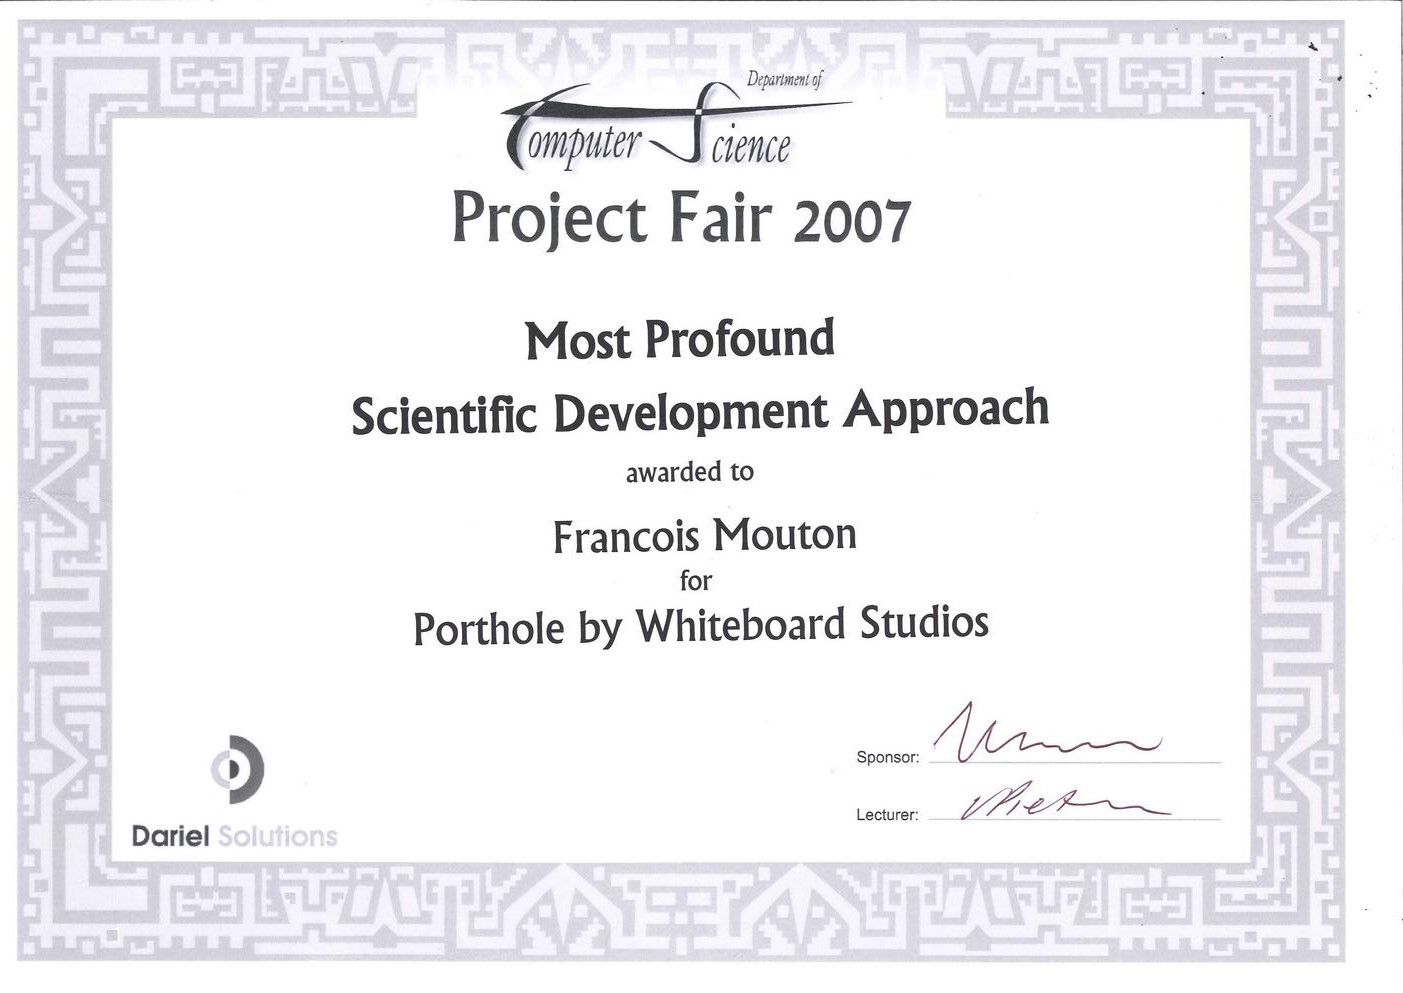
\includepdf[pages=-]{appendix/Project_Fair_2007_Most_Profound_Scientific_Development_Approach.jpg}

\phantomsection\addcontentsline{toc}{subsection}{Business Opportunity Award}
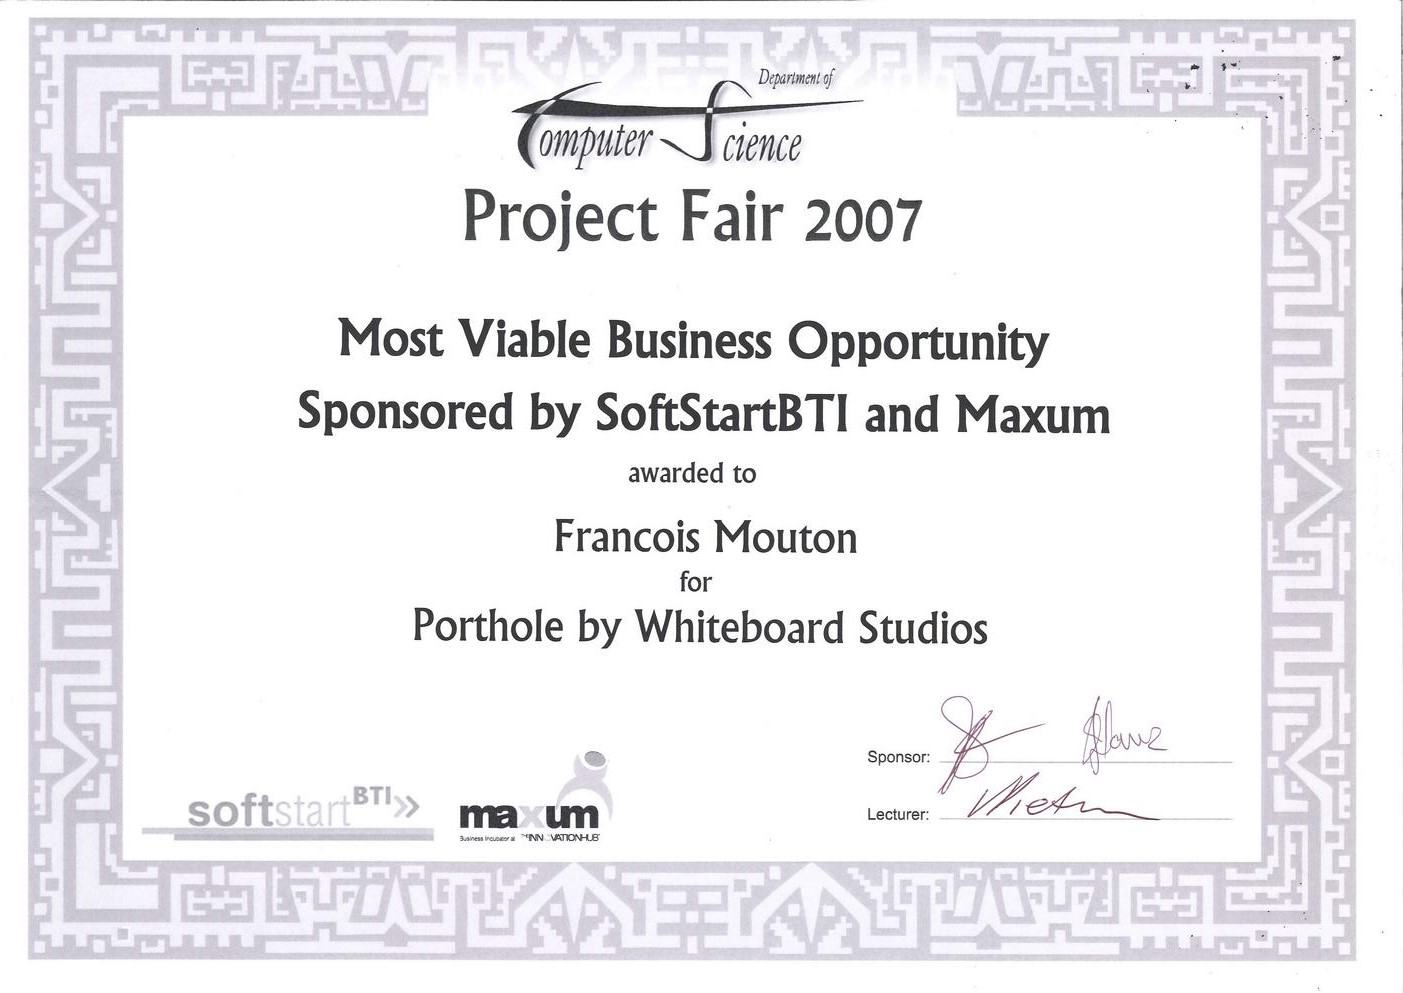
\includepdf[pages=-]{appendix/Project_Fair_2007_Most_Viable_Business_Opportunity.jpg}

\phantomsection
\addcontentsline{toc}{section}{Other}

\phantomsection
\addcontentsline{toc}{subsection}{Golden Key}

\includepdf[pages=-]{appendix/Golden_Key_International_Honour_Society.jpg}

\phantomsection
\addcontentsline{toc}{subsection}{Senior Certificate}
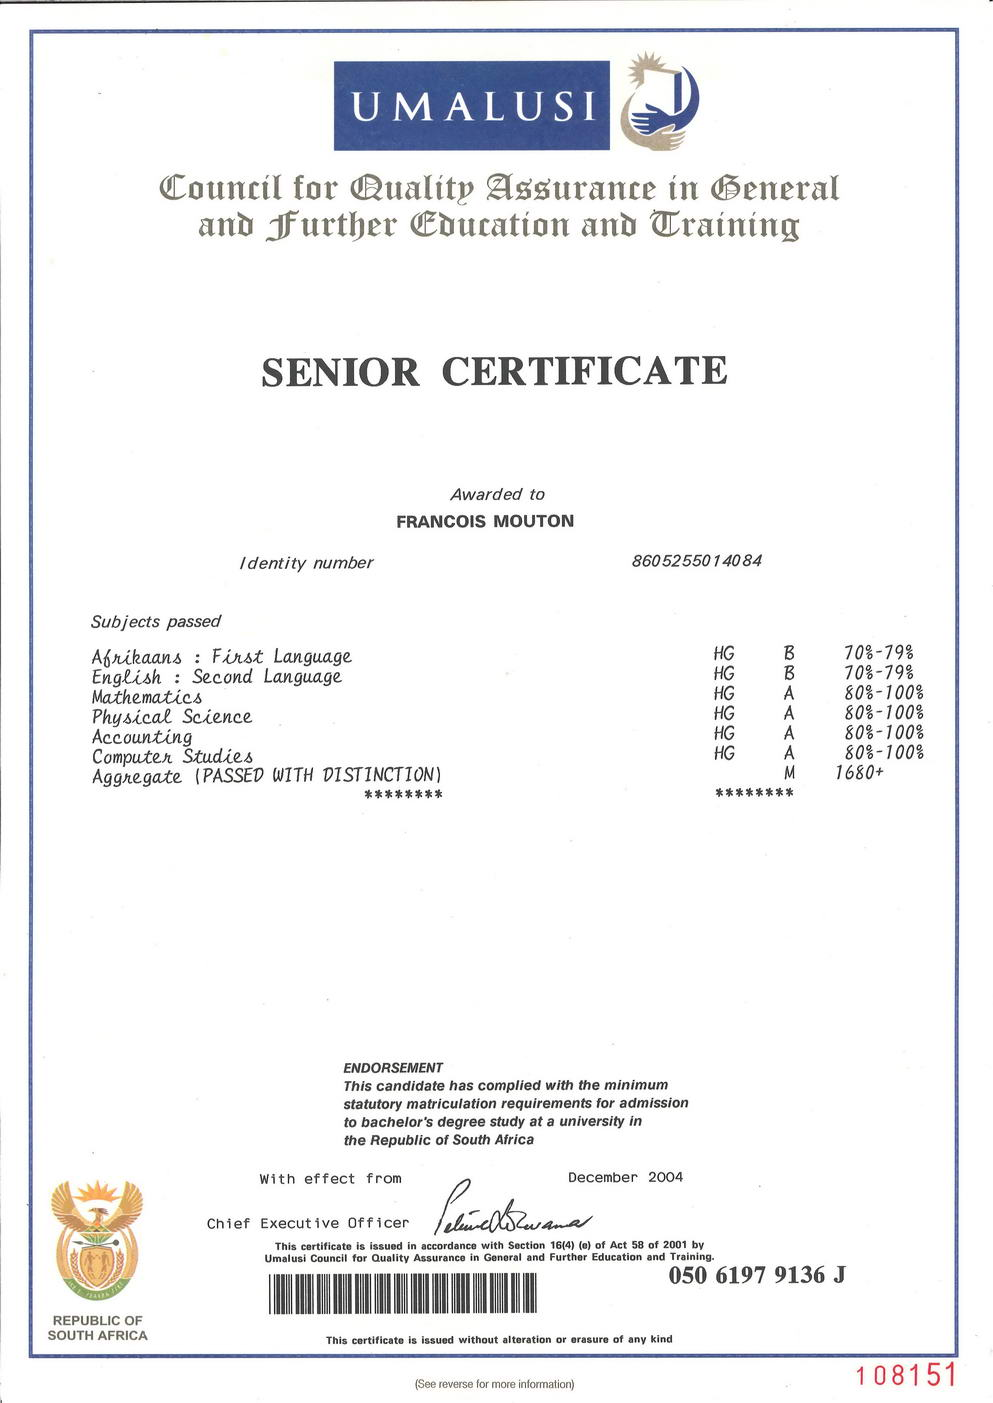
\includepdf[pages=-]{appendix/Senior_Certificate.jpg}

\phantomsection
\addcontentsline{toc}{subsection}{Top Student Award}

\includepdf[pages=-]{appendix/TopStudent2006.jpg}

\phantomsection
\addcontentsline{toc}{subsection}{IFIP Wireless Computing}
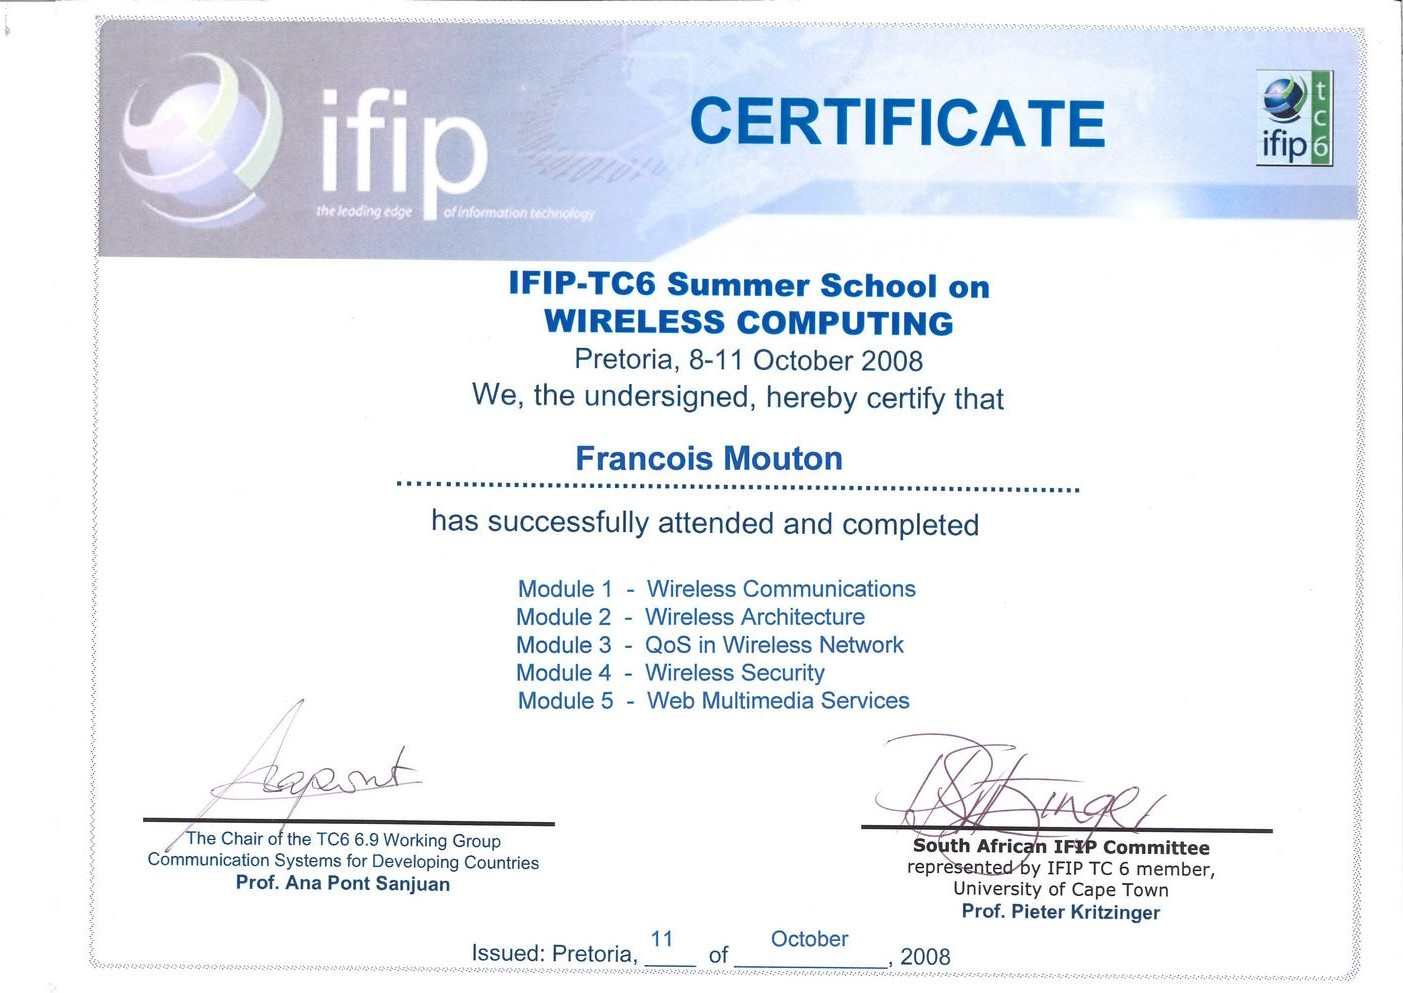
\includepdf[pages=-]{appendix/IFIP_Wireless_Computing.jpg}

%-------------------Document End------------------------------------------------------------------------

\end{document}

%% end of file `main.tex'.
